\subsection{Méthode des facteurs de faux ou \emph{fake factors}}\label{chapter-HTT_analysis-section-bg_estimation-FF_method}
La méthode des facteurs de faux (\emph{fake factors}) a pour but de fournir, en se basant presque exclusivement sur les données collectées, une estimation des bruits de fond dans lesquels des jets, provenant de quarks ou de gluons, sont identifiés à tort comme des taus hadroniques (\tauh).
De tels jets sont notés \og \ftauh \fg{} dans la suite.
\par
Cette méthode est ainsi appliquée aux canaux contenant des \tauh\ dans l'état final, \ie\ les canaux complètement hadronique (\tauh\tauh) et semi-leptoniques ($\ell\tauh$ où $\ell\in\set{\ele,\mu}$).
Les \ftauhs\ représentent près de \SI{70}{\%} des événements dans le canal \tauh\tauh, \SI{38}{\%} dans le canal \mu\tauh\ et \SI{68}{\%} dans le canal \ele\tauh~\cite{CMS-NOTE-2018-257,CMS-NOTE-2019-170}.
Les processus physiques responsables des \ftauhs\ sont majoritairement QCD, \Wjets\ et \ttbar.
Dans le canal \tauh\tauh, près de \SI{93}{\%} des \ftauhs\ proviennent du bruit de fond QCD.
Dans les canaux $\ell\tauh$, environ \SI{70}{\%} des \ftauhs\ sont issus du bruit de fond \Wjets.
Les autres sources de \ftauhs, non traités par cette méthode, sont les événements $\Zboson\to\tau\tau$ avec un jet identifié comme un \tauh, couverts par la méthode décrite section~\ref{chapter-HTT_analysis-section-bg_estimation-embedding}, et Diboson, ce dernier type de processus ne contribuant que de l'ordre du pourcent au total des \ftauhs.
\par
Les \ftauhs\ sont particulièrement difficiles à modéliser dans les simulations~\cite{CMS-NOTE-2018-257,CMS-NOTE-2019-170}.
De plus, le faible de taux de mauvaise identification des \tauh, inférieur à \SI{1}{\%}, impliquerait l'utilisation de larges jeux de données simulées afin d'obtenir de faibles incertitudes statistiques.
C'est en particulier le cas dans les régions de l'espace des phases contenant des bosons de Higgs lourds, ce que recherche cette analyse.
La méthode des \fakefactors\ se basant presque exclusivement sur les données collectées, les incertitudes inhérentes aux simulations deviennent négligeables face aux autres sources d'incertitudes.
De plus, l'efficacité statistique de cette modélisation est directement liée à la luminosité intégrée, sans nécessiter de données simulées correspondantes.
\subsubsection{Principe de base}
Cette méthode suit le même principe de produit en croix que la méthode \og ABCD \fg{} présentée section~\ref{chapter-HTT_analysis-section-bg_estimation-QCD-SS} mais va plus loin dans la détermination du facteur $C/D$ nommé ici \fakefactor.
Dans une région de contrôle, détaillée dans la section suivante, le rapport des quantités de \tauh\ isolés sur ceux anti-isolés est déterminé.
Il s'agit du \fakefactor\, noté \FF, défini comme
\begin{equation}
\FF = \frac{n_\text{iso}}{n_\text{anti-iso}} = \frac{n(\texttt{Medium})}{n(\texttt{VVVLoose \&\& !Medium})}
\label{eq-chapter-HTT_analysis-section-bg_estimation-FF_method-FF_def_global}
\end{equation}
où
\begin{itemize}
\item $n(\texttt{Medium})$ est la quantité d'événements dans la région de contrôle (CR, \emph{Control Region}) passant le point de fonctionnement \PassDeepTau{moyen}{medium}{vs jet}, utilisé également pour sélectionner les événements de signal;
\item $n(\texttt{VVVLoose \&\& !Medium})$ est la quantité d'événements dans la région de contrôle passant le point de fonctionnement le plus lâche de ce discriminateur, mais pas le moyen.
\end{itemize}
Le \fakefactor\ \FF\ est déterminé de manière indépendante pour chaque canal (\tauh\tauh, \mu\tauh, \ele\tauh), chaque année (2016, 2017, 2018) et dépend:
\begin{itemize}
\item de l'impulsion transverse de l'objet physique identifié comme un \tauh, $\pT^{\tauh}$;
\item de l'impulsion transverse du jet le plus proche du \tauh, $\pT^\text{jet}$;
\item du nombre de jets tels que $\abs{\eta^\text{jet}}<\num{2.4}$ et $\pT^\text{jet}>\SI{20}{\GeV}$, \Nprebjets.
\end{itemize}
\par
Une région d'application du \fakefactor\ (AR, \emph{Application Region}) est définie de manière similaire à la région de signal (SR, \emph{Signal Region}), seul le critère d'isolation des \tauh\ passe de \og isolé \fg{}  à \og anti-isolé \fg.
La AR est ainsi riche en \ftauhs.
La quantité d'événements contenant des \ftauhs\ dans la SR, notée $n_{j\to\tauh}$, est alors obtenue par produit en croix avec la quantité d'événements dans la AR, notée $n_\text{AR}$,  selon
\begin{equation}
n_{j\to\tauh} = n_\text{AR} \cdot \FF
\mend[,]
\end{equation}
l'hypothèse étant l'universalité, \ie\ que le \fakefactor\ mesuré dans la CR est supposé identique à celui de la AR.
\subsubsection{Prise en compte des différentes sources de \ftauhs}
La composition des jets n'est pas la même selon le processus physique dont proviennent les \ftauhs.
Il existe donc différentes probabilités pour un jet de donner un \ftauh.
Dans le cas du canal \tauh\tauh, seul le bruit de fond QCD est traité par les \fakefactors.
Pour les canaux semi-leptoniques, trois sources de \ftauhs\ sont considérées, QCD, \Wjets\ et \ttbar.
Pour chacune de ces sources, un \fakefactor\ est alors déterminé, selon l'équation~\eqref{eq-chapter-HTT_analysis-section-bg_estimation-FF_method-FF_def_global}, à partir d'une région de détermination (DR, \emph{Determination Region}) dédiée, définie ci-après.
Du fait de la séparation de la CR en plusieurs DR, l'universalité n'est alors plus complètement garantie.
Des corrections résiduelles sont appliquées afin de corriger le biais introduit par la séparation en DR.
\par
Le \fakefactor\ global est ainsi la moyenne des \fakefactors\ obtenus pour chaque source, avec comme coefficients les fractions $f$ d'événements de ces sources dans la AR, \ie
\begin{equation}
\FF = \sum_i f_i \cdot \FF_i
\msep
f_i = \frac{n_\text{AR}^i}{\sum_j n_\text{AR}^{j}}
\msep
i,j \in \set{\text{QCD, \Wjets, \ttbar}}
\mend
\end{equation}
Les fractions $f_i$ sont déterminées à partir de simulations et dépendent:
\begin{itemize}
\item de la masse transverse du lepton $\ell\in\set{\ele,\mu}$, $\mT^{\ell}$;
\item du nombre de jets \Nprebjets\ identifiés comme issus de quarks~\quarkb, \Nbjets;
\item de la masse transverse totale, définie équation~\eqref{eq-def_mTtot}, \mTtot.
\end{itemize}
La figure~\ref{fig-chapter-HTT_analysis-section-bg_estimation-FF_method-fractions} présente ces fractions en fonction de \mTtot\ pour $\mT^{\mu} < \SI{40}{\GeV}$ et $\Nbjets\in\set{0,\geq1}$ pour le canal \mu\tauh\ en 2018.
La méthode des \fakefactors\ est résumée figure~\ref{fig-chapter-HTT_analysis-section-bg_estimation-FF_method-ppe}.
\begin{figure}[h]
\centering

\subcaptionbox{Pour $\Nbjets=0$ et $\mT^{\mu} < \SI{40}{\GeV}$}[.45\textwidth]
{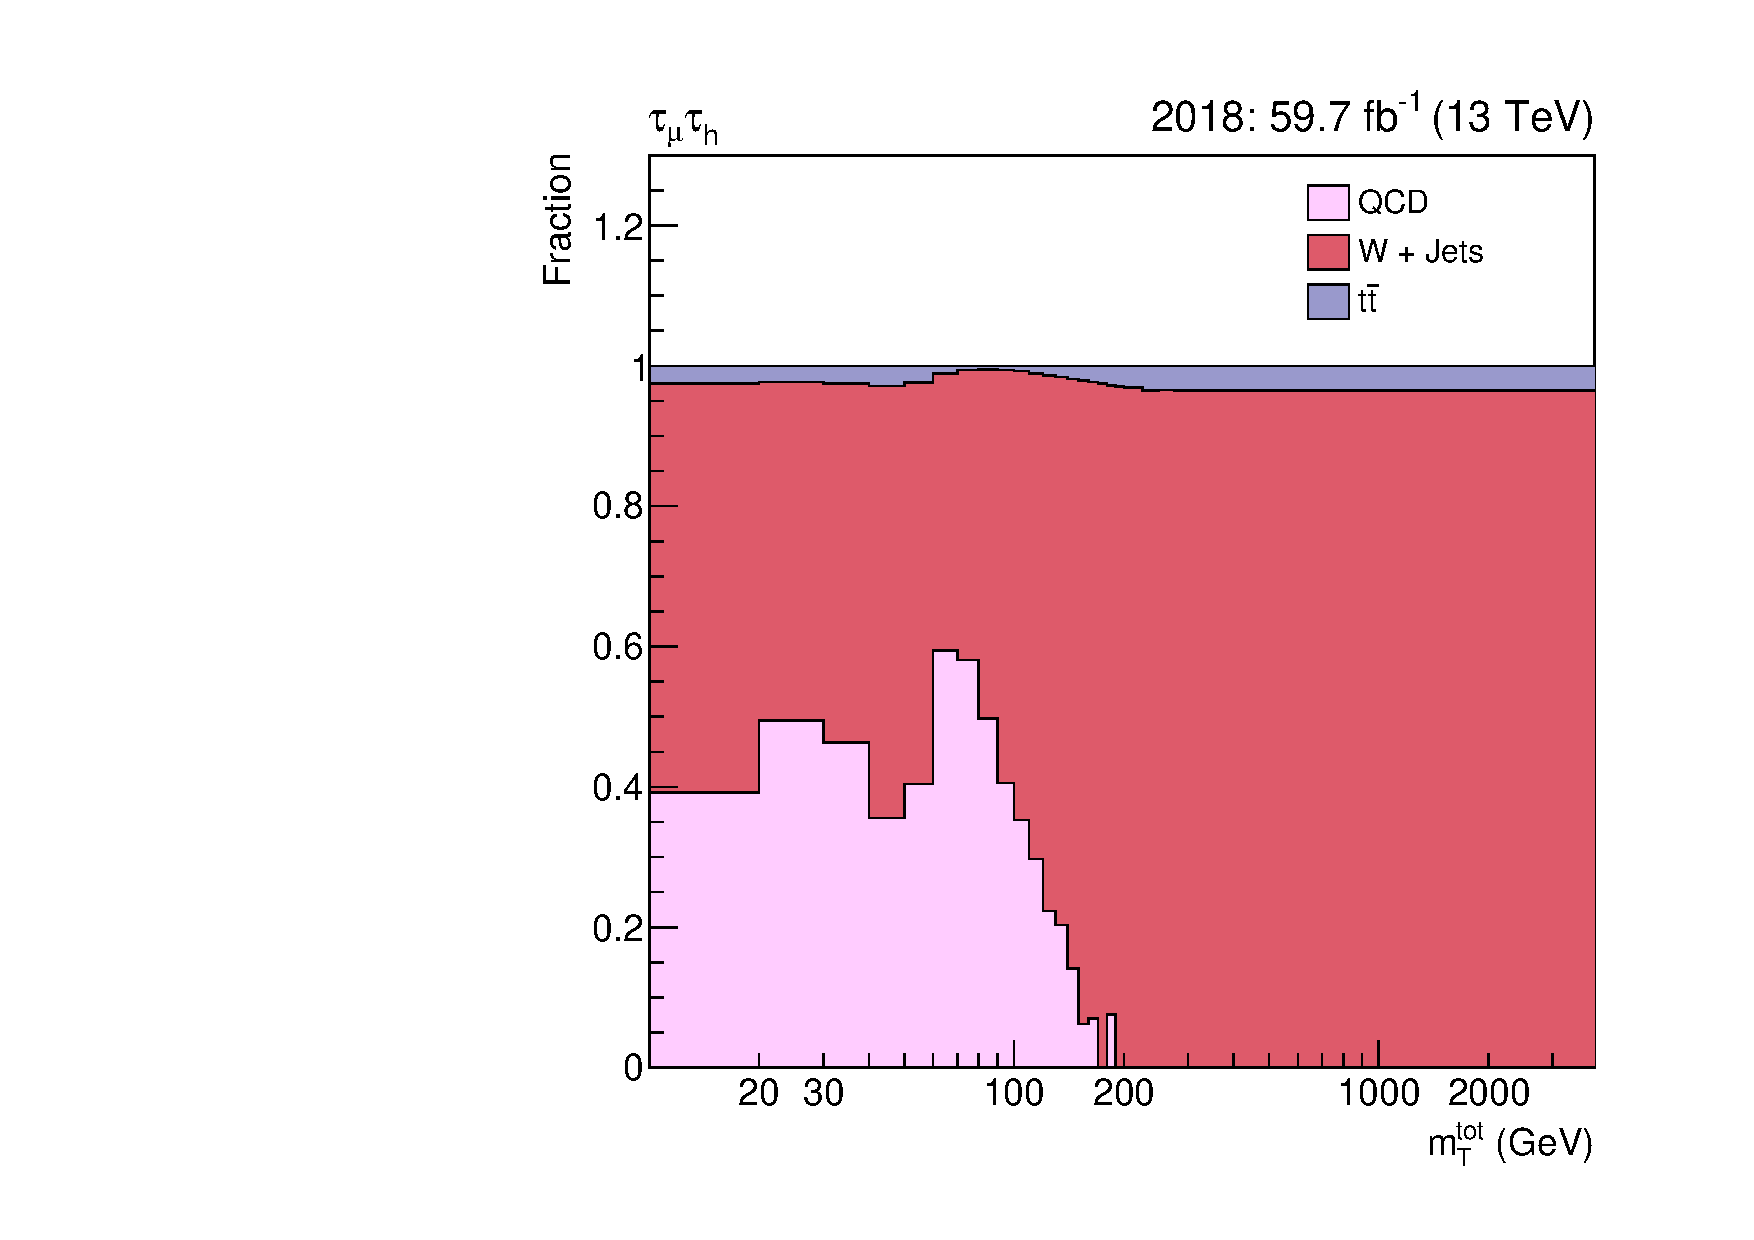
\includegraphics[width=.45\textwidth]{\PhDthesisdir/plots_and_images/from_CMS-NOTE-2020-218/ff_fraction_tightmt_nbjets0_mt_2018_os_rebinning.tex}}
\hfill
\subcaptionbox{Pour $\Nbjets\geq1$ et $\mT^{\mu} < \SI{40}{\GeV}$}[.45\textwidth]
{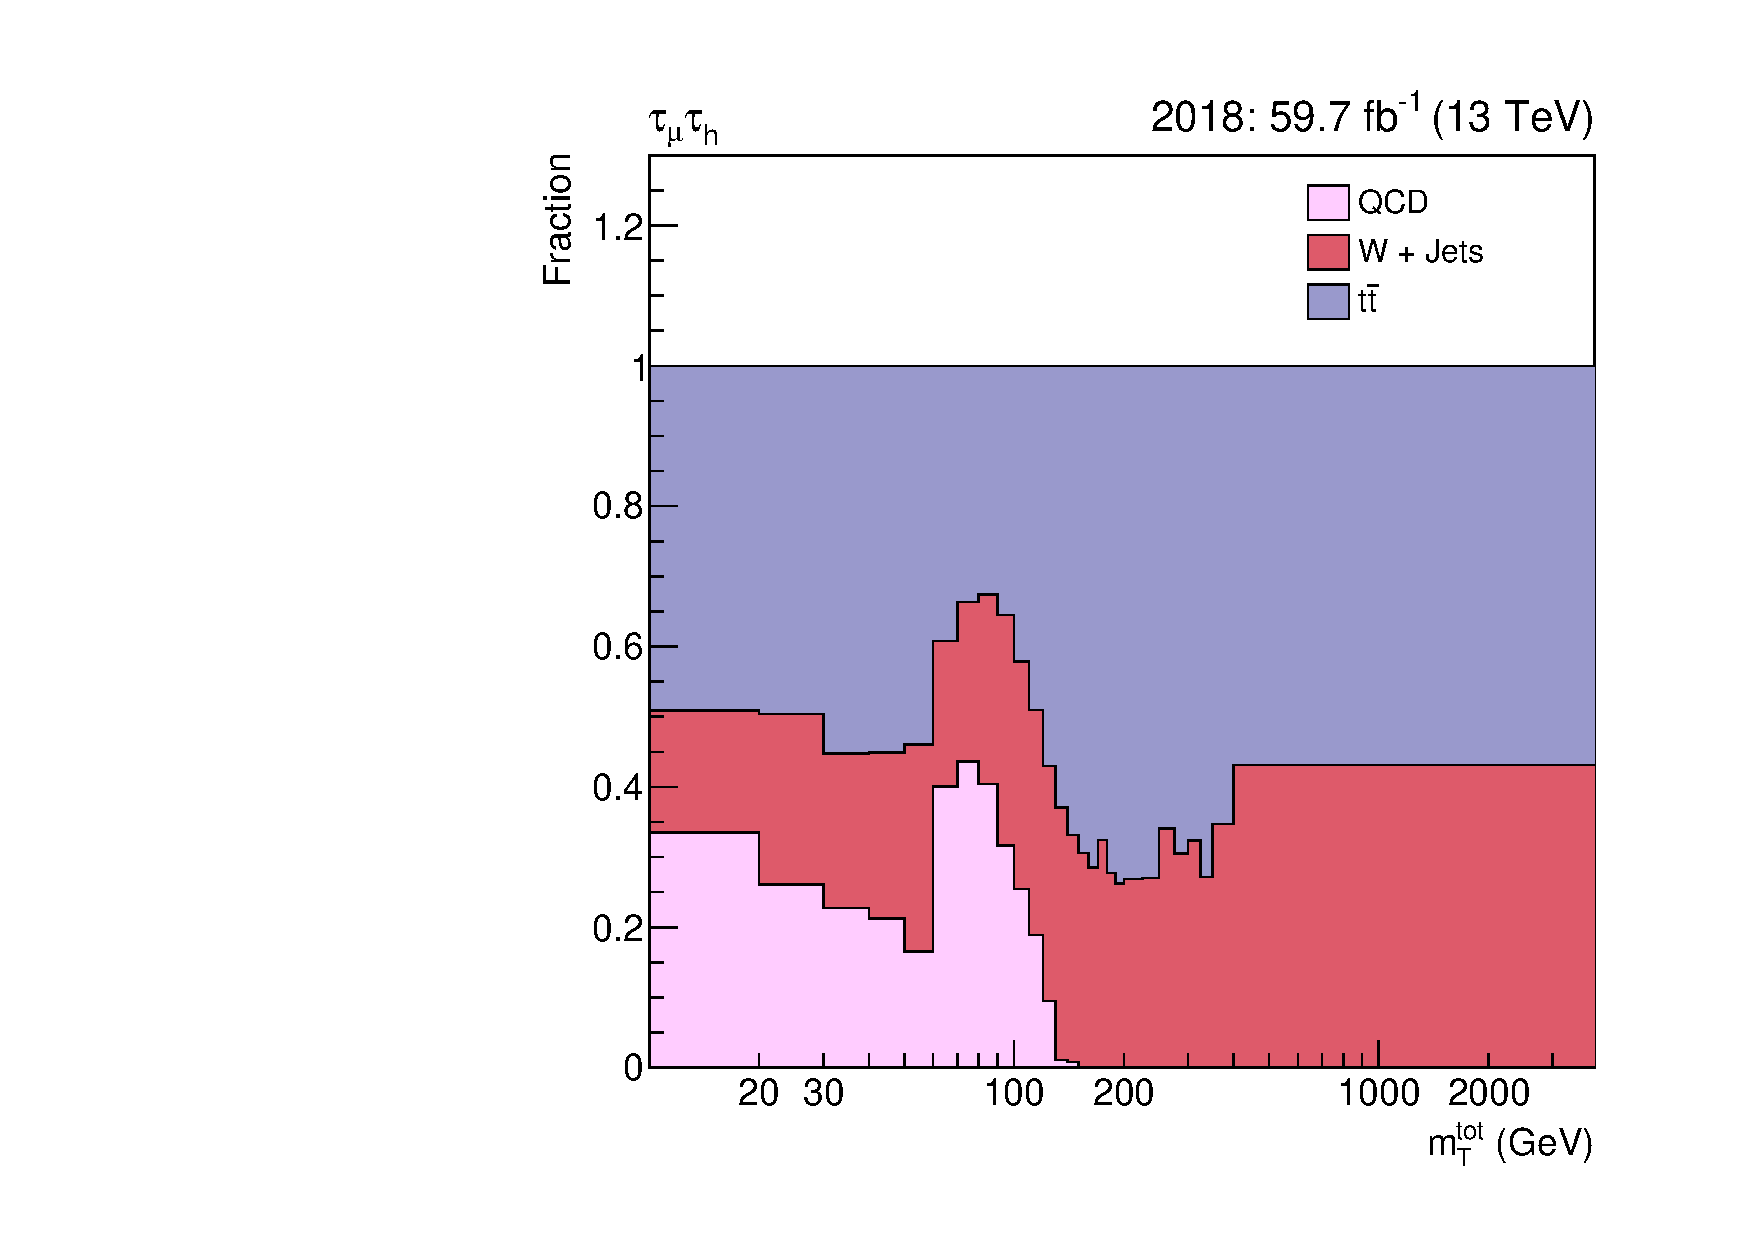
\includegraphics[width=.45\textwidth]{\PhDthesisdir/plots_and_images/from_CMS-NOTE-2020-218/ff_fraction_tightmt_nbjets1_mt_2018_os_rebinning.tex}}

\caption[Fractions des sources de \ftauhs\ dans le canal \mu\tauh\ en 2018.]{Fractions des sources de \ftauhs\ dans le canal \mu\tauh\ en 2018~\cite{CMS-NOTE-2020-218}.}
\label{fig-chapter-HTT_analysis-section-bg_estimation-FF_method-fractions}
\end{figure}
\begin{figure}[h]
\centering
\begin{tikzpicture}
\def\RegionW{3}
\def\RegionH{2.5}

\fill [ltcolorgray2] (0,0) rectangle + (\RegionW,\RegionH);
\fill [ltcolorred2] (\RegionW,0) rectangle + (\RegionW,\RegionH);
\fill [ltcolormagenta2] (2*\RegionW,0) rectangle + (\RegionW,\RegionH);
\fill [ltcolorviolet2] (3*\RegionW,0) rectangle + (\RegionW,\RegionH);

\fill [ltcolorgray1] (0,\RegionH) rectangle + (\RegionW,\RegionH);
\fill [ltcolorred1] (\RegionW,\RegionH) rectangle + (\RegionW,\RegionH);
\fill [ltcolormagenta1] (2*\RegionW,\RegionH) rectangle + (\RegionW,\RegionH);
\fill [ltcolorviolet1] (3*\RegionW,\RegionH) rectangle + (\RegionW,\RegionH);

\draw [ultra thick, -latex] (0.875*\RegionW, \RegionH-\RegionW/6) --+ (0,\RegionW/3);

%\draw (1.5*\RegionW, \RegionH) node [above] (FFW) {\Large $\FF_\Wboson$};
%\draw (2.5*\RegionW, \RegionH) node [above] (FFQ) {\Large $\FF_Q$};
%\draw (3.5*\RegionW, \RegionH) node [above] (FFT) {\Large $\FF_\quarkt$};

\foreach \value/\DeterminationRegion/\nodecoord in {1.5/\Wboson/FFW, 2.5/Q/FFQ, 3.5/\quarkt/FFT}{
\draw (\value*\RegionW, \RegionH) node (\nodecoord) {\large $\displaystyle \FF_{\DeterminationRegion}=\frac{n_\text{iso}^{\DeterminationRegion}}{n_\text{anti-iso}^{\DeterminationRegion}}$};
}

\draw [ultra thick] (1*\RegionW,1.4*\RegionH)  to [out=0,in=90, out looseness = 1.5, in looseness = 1] (5*\RegionW/4,8*\RegionH/7);
\draw [ultra thick] (2*\RegionW,1.4*\RegionH)  to [out=0,in=90, out looseness = 1.5, in looseness = 1] (9*\RegionW/4,8*\RegionH/7);

\draw [ultra thick, latex-] (.9*\RegionW,1.4*\RegionH) -- (3*\RegionW,1.4*\RegionH)  to [out=0,in=90, out looseness = 1.5, in looseness = 1] (13*\RegionW/4,8*\RegionH/7);

\draw [thick, -latex] (-\RegionW/5,0) -- (4*\RegionW,0) --+ (\RegionW/5,0) node [right] {Région};
\draw [thick, -latex] (0,-\RegionW/5) -- (0,2*\RegionH) --+ (0,\RegionW/5) node [above] {Isolation du \tauh};

\draw (-0*\RegionW, 1.5*\RegionH) node [above, rotate=90] {isolé};

\draw (-0*\RegionW, .5*\RegionH) node [above, rotate=90] {anti-isolé};

\draw (.45*\RegionW, .675*\RegionH) node {\small fractions des};
\draw (.45*\RegionW, .525*\RegionH) node {\small processus};
\draw (\RegionW, .6*\RegionH) node [left] {$\mathrm{f}_i$};

\draw (.45*\RegionW, .275*\RegionH) node {\small quantité};
\draw (.45*\RegionW, .125*\RegionH) node {\small d'événements};
\draw (\RegionW, .2*\RegionH) node [left] {$n_\text{AR}$};


\draw (.5*\RegionW, 1.65*\RegionH) node {$n_\text{AR}\cdot\sum_i f_i \cdot \FF_i$\ };
\draw (.5*\RegionW, 1.4*\RegionH) node {$=n_{j\to\tauh}$};

\draw (.5*\RegionW, 2*\RegionH) node [below] {\textbf{SR}};
\draw (.5*\RegionW, 1*\RegionH) node [below] {\textbf{AR}};

% $\Wboson+\text{jets}$, QCD multijet, $\ttbar+\text{jets}$

\draw (0.5*\RegionW, 0) node [below] {AR \& SR} ;
\draw (1.5*\RegionW, 0) node [below] {DR \Wjets} ;
\draw (2.5*\RegionW, 0) node [below] {DR QCD} ;
\draw (3.5*\RegionW, 0) node [below] {DR \ttbar} ;

\end{tikzpicture}
\caption[Illustration de la méthode des \fakefactors.]{Illustration de la méthode des \fakefactors. Les \fakefactors\ sont obtenus à partir du nombre d'événements avec des \tauh\ isolés et anti-isolés dans les régions de détermination (DR) de chaque processus contribuant significativement au bruit de fond contenant des \ftauhs. La quantité de \ftauhs\ dans la région de signal (SR) est estimée à partir des fractions de ces processus et du nombre d'événements présents dans la région d'application (AR).}
\label{fig-chapter-HTT_analysis-section-bg_estimation-FF_method-ppe}
\end{figure}
\subsubsection{Régions de détermination}
\paragraph{QCD}
La DR QCD est définie de la même manière que la SR à l'exception du critère sur les charges électriques des éléments du \emph{dilepton}.
En effet, ceux-ci doivent être de charges opposées (OS, \emph{Opposite Signs}) dans la SR car les bosons de Higgs recherchés étant neutres, la charge globale du \emph{dilepton} doit, par conservation, être nulle.
Pour la DR QCD, ces charges doivent être de même signe (SS, \emph{Same Sign}).
Dans le cas des canaux $\ell\tauh$, il est de plus requis que $I_\text{rel}^{\ell} > \num{0.05}$ afin de réduire les contribution de processus donnant des électrons ou des muons sans objet physique pertinent pour les \fakefactors.
Les contributions d'autres processus à la DR est soustraite grâce à l'utilisation de données simulées.
Pour le canal \tauh\tauh, le \fakefactor\ $\FF_Q$ est déterminé uniquement pour le premier \tauh\ (de plus haut \pT).
\par
Le \fakefactor\ $\FF_Q$ est mesuré séparément pour:
\begin{itemize}
\item $\Nprebjets=0$;
\item $\Nprebjets\geq1$;
\end{itemize}
et dans chacun de ces deux cas pour
\begin{itemize}
\item $\pT^\text{jet}/\pT^{\tauh} < \num{1.25}$;
\item $\num{1.25} \leq \pT^\text{jet}/\pT^{\tauh} < \num{1.5}$;
\item $\num{1.5} \leq \pT^\text{jet}/\pT^{\tauh}$.
\end{itemize}
Pour ces six catégories, la dépendance en $\pT^{\tauh}$ de $\FF_Q$ est modélisée polynôme de degré 3 ajusté aux mesures pour $\pT^{\tauh}<\SI{200}{\GeV}$.
\par
Dans le cas du canal \tauh\tauh, peu d'événements sont disponibles pour $\pT^{\tauh}\geq\SI{200}{\GeV}$.
Le \fakefactor\ $\FF_Q$ est ainsi fixé à la valeur mesurée pour $\pT^\text{jet}/\pT^{\tauh} \geq \num{1.5}$ et à la valeur à \SI{200}{\GeV} du polynôme pour $\pT^\text{jet}/\pT^{\tauh} < \num{1.5}$.
Pour les canaux $\ell\tauh$, la situation est similaire à partir de $\pT^{\tauh}\geq\SI{140}{\GeV}$.
La valeur utilisée à haut $\pT^{\tauh}$ suit la logique suivante:
\begin{itemize}
\item si l'erreur relative sur $\FF_Q$ pour $\pT^{\tauh}\geq\SI{200}{\GeV}$ est inférieure à \num{0.5}:
\begin{itemize}
\item si l'erreur relative sur $\FF_Q$ pour $\pT^{\tauh}\in[140, 200]\usp\SI{}{\GeV}$ est inférieure à \num{0.5}, les valeurs mesurées sont utilisées sur les intervalles $[140, 200]\usp\SI{}{\GeV}$ et $[200, \infty[\usp\SI{}{\GeV}$,
\item si l'erreur relative sur $\FF_Q$ pour $\pT^{\tauh}\in[140, 200]\usp\SI{}{\GeV}$ est supérieure à \num{0.5}, la valeur mesurée est utilisée sur l'intervalle $[200, \infty[\usp\SI{}{\GeV}$;
\end{itemize}
\item si l'erreur relative sur $\FF_Q$ pour $\pT^{\tauh}\geq\SI{200}{\GeV}$ est supérieure à \num{0.5}
et inférieure à \num{0.5} pour $\pT^{\tauh}\in[140, 200]\usp\SI{}{\GeV}$,
la valeur mesurée est utilisée sur l'intervalle $[140, \infty[\usp\SI{}{\GeV}$;
\item sinon, la valeur obtenue par l'ajustement est utilisée.
\end{itemize}
%L'ajustement obtenu pour $\FF_Q$ sur le canal \mu\tauh\ en 2018 est illustré figure~\ref{fig-chapter-HTT_analysis-section-bg_estimation-FF_method-FFQ_fit} pour $\Nprebjets=0$ et $\num{1.5} \leq \pT^\text{jet}/\pT^{\tauh}$.
%\begin{figure}[h]
%\centering
%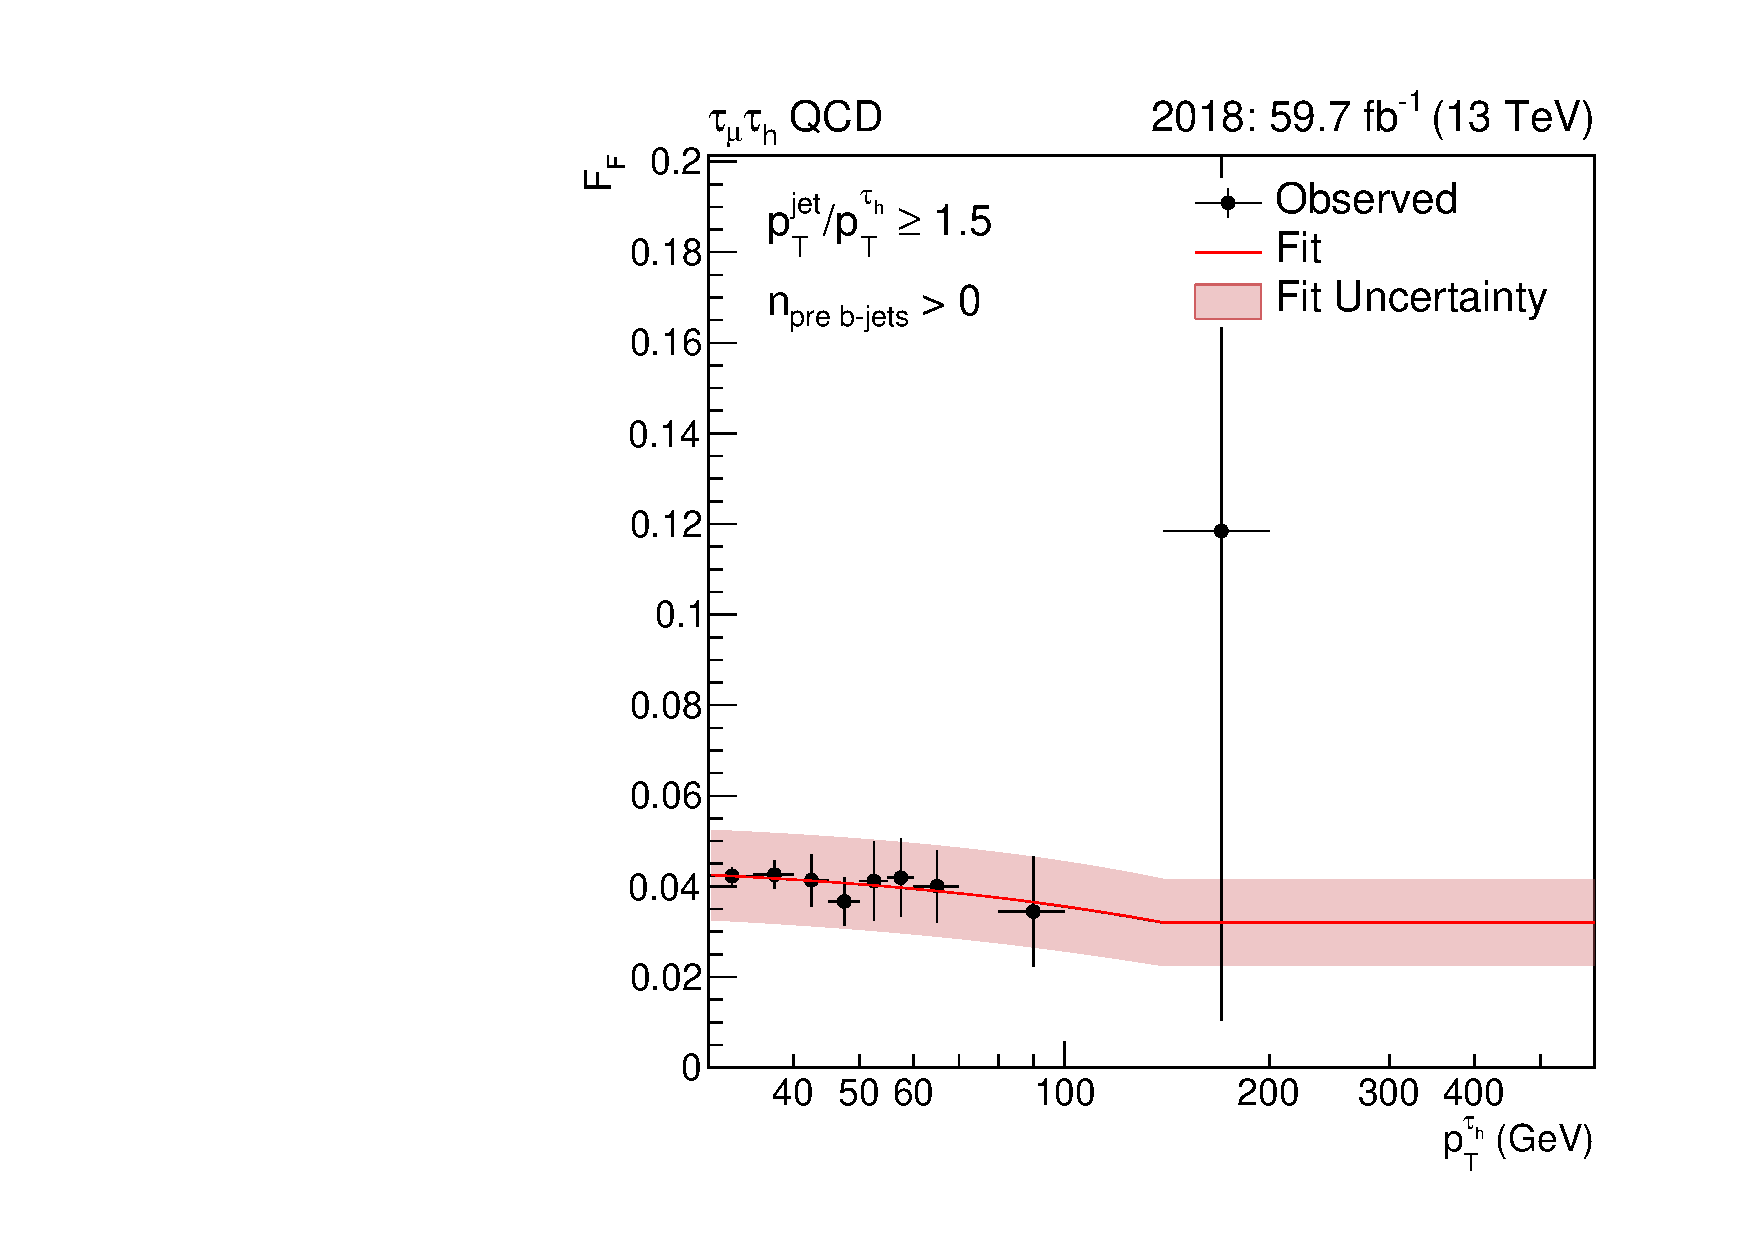
\includegraphics[width=.45\textwidth]{\PhDthesisdir/plots_and_images/from_CMS-NOTE-2020-218/ff_fit_jet_pt_high_1jet_pt_2_ff_qcd_mt_2018.tex}
%\caption[Ajustement de $\FF_Q$ dans le canal \mu\tauh\ en 2018.]{Ajustement de $\FF_Q$ dans le canal \mu\tauh\ en 2018~\cite{CMS-NOTE-2020-218}.}
%\label{fig-chapter-HTT_analysis-section-bg_estimation-FF_method-FFQ_fit}
%\end{figure}
\paragraph{\Wjets}
La DR \Wjets\ ne concerne que les canaux semi-leptoniques.
Elle est définie de la même manière que la SR à l'exception de la coupure sur la masse transverse du lepton qui doit ici être supérieure à \SI{70}{\GeV}, alors qu'elle est inférieure à cette même valeur dans la SR.
Il est de plus requis que $\Nbjets=0$ afin de supprimer la contamination par les événements \ttbar.
Les contributions d'autres processus physiques à la DR sont soustraites par l'utilisation directe de données simulées.
Le bruit de fond QCD à retirer est obtenu à partir des données réelles avec les charges électriques des éléments du \emph{dilepton} de même signe, auxquelles sont soustraites les autres bruits de fond avec charges électriques de même signe, y compris \Wjets, obtenus par simulation directe.
Un facteur correctif de \num{1.1} est appliqué aux données à retirer, correspondant au rapport observé d'événements avec charges opposées sur événements avec charges de même signe.
\par
Le \fakefactor\ $\FF_W$ est mesuré séparément pour:
\begin{itemize}
\item $\Nprebjets=0$;
\item $\Nprebjets\geq1$;
\end{itemize}
et dans chacun de ces deux cas pour
\begin{itemize}
\item $\pT^{\text{jet})}/\pT^{\tauh} < \num{1.25}$;
\item $\num{1.25} \leq \pT^\text{jet}/\pT^{\tauh} < \num{1.5}$;
\item $\num{1.5} \leq \pT^\text{jet}/\pT^{\tauh}$.
\end{itemize}
Pour ces six catégories, la dépendance en $\pT^{\tauh}$ de $\FF_Q$ est modélisée polynôme de degré 3 ajusté aux mesures pour $\pT^{\tauh}<\SI{140}{\GeV}$.
\par
Dans cette DR également, peu d'événements sont disponibles pour $\pT^{\tauh}\geq\SI{140}{\GeV}$.
La même logique que pour $\FF_Q$, détaillée précédemment, est suivie sur la valeur de $\FF_W$ à utiliser.
L'ajustement obtenu pour $\FF_W$ sur le canal \mu\tauh\ en 2018 est illustré figure~\ref{subfig-chapter-HTT_analysis-section-bg_estimation-FF_method-WJ} pour $\Nprebjets\geq1$ et $\num{1.25} \leq \pT^\text{jet}/\pT^{\tauh} < \num{1.5}$.
Il y apparaît l'effet du traitement de la région à haut $\pT^{\tauh}$.
\paragraph{\ttbar}
La DR \ttbar\ ne concerne que les canaux semi-leptoniques.
Il n'est pas possible de définir une DR issue des données suffisamment pure pour mesurer $\FF_t$.
Ce \fakefactor\ est alors obtenu à partir de données simulées.
\par
Le \fakefactor\ $\FF_W$ peut également être mesuré à partir de données simulées uniquement.
Un écart de \num{10} à \SI{20}{\%} avec le \fakefactor\ obtenu à partir des données réelles est observé.
La contribution \ttbar\ étant faible par rapport aux autres bruits de fond rend négligeable le biais introduit par l'utilisation de données simulées face aux incertitudes sur les \fakefactors.
\par
Le \fakefactor\ $\FF_t$ est mesuré séparément pour:
\begin{itemize}
\item $\pT^\text{jet}/\pT^{\tauh} < \num{1.25}$;
\item $\num{1.25} \leq \pT^\text{jet}/\pT^{\tauh} < \num{1.5}$;
\item $\num{1.5} \leq \pT^\text{jet}/\pT^{\tauh}$;
\end{itemize}
sans séparation en \Nprebjets, la majorité des événements \ttbar\ vérifiant $\Nprebjets\geq1$.
L'ajustement obtenu pour $\FF_t$ sur le canal \mu\tauh\ en 2018 est illustré figure~\ref{subfig-chapter-HTT_analysis-section-bg_estimation-FF_method-ttbar} pour $\pT^\text{jet}/\pT^{\tauh} < \num{1.25}$.
\begin{figure}[h]
\centering

\subcaptionbox{Ajustement de $\FF_W$.\label{subfig-chapter-HTT_analysis-section-bg_estimation-FF_method-WJ}}[.45\textwidth]
{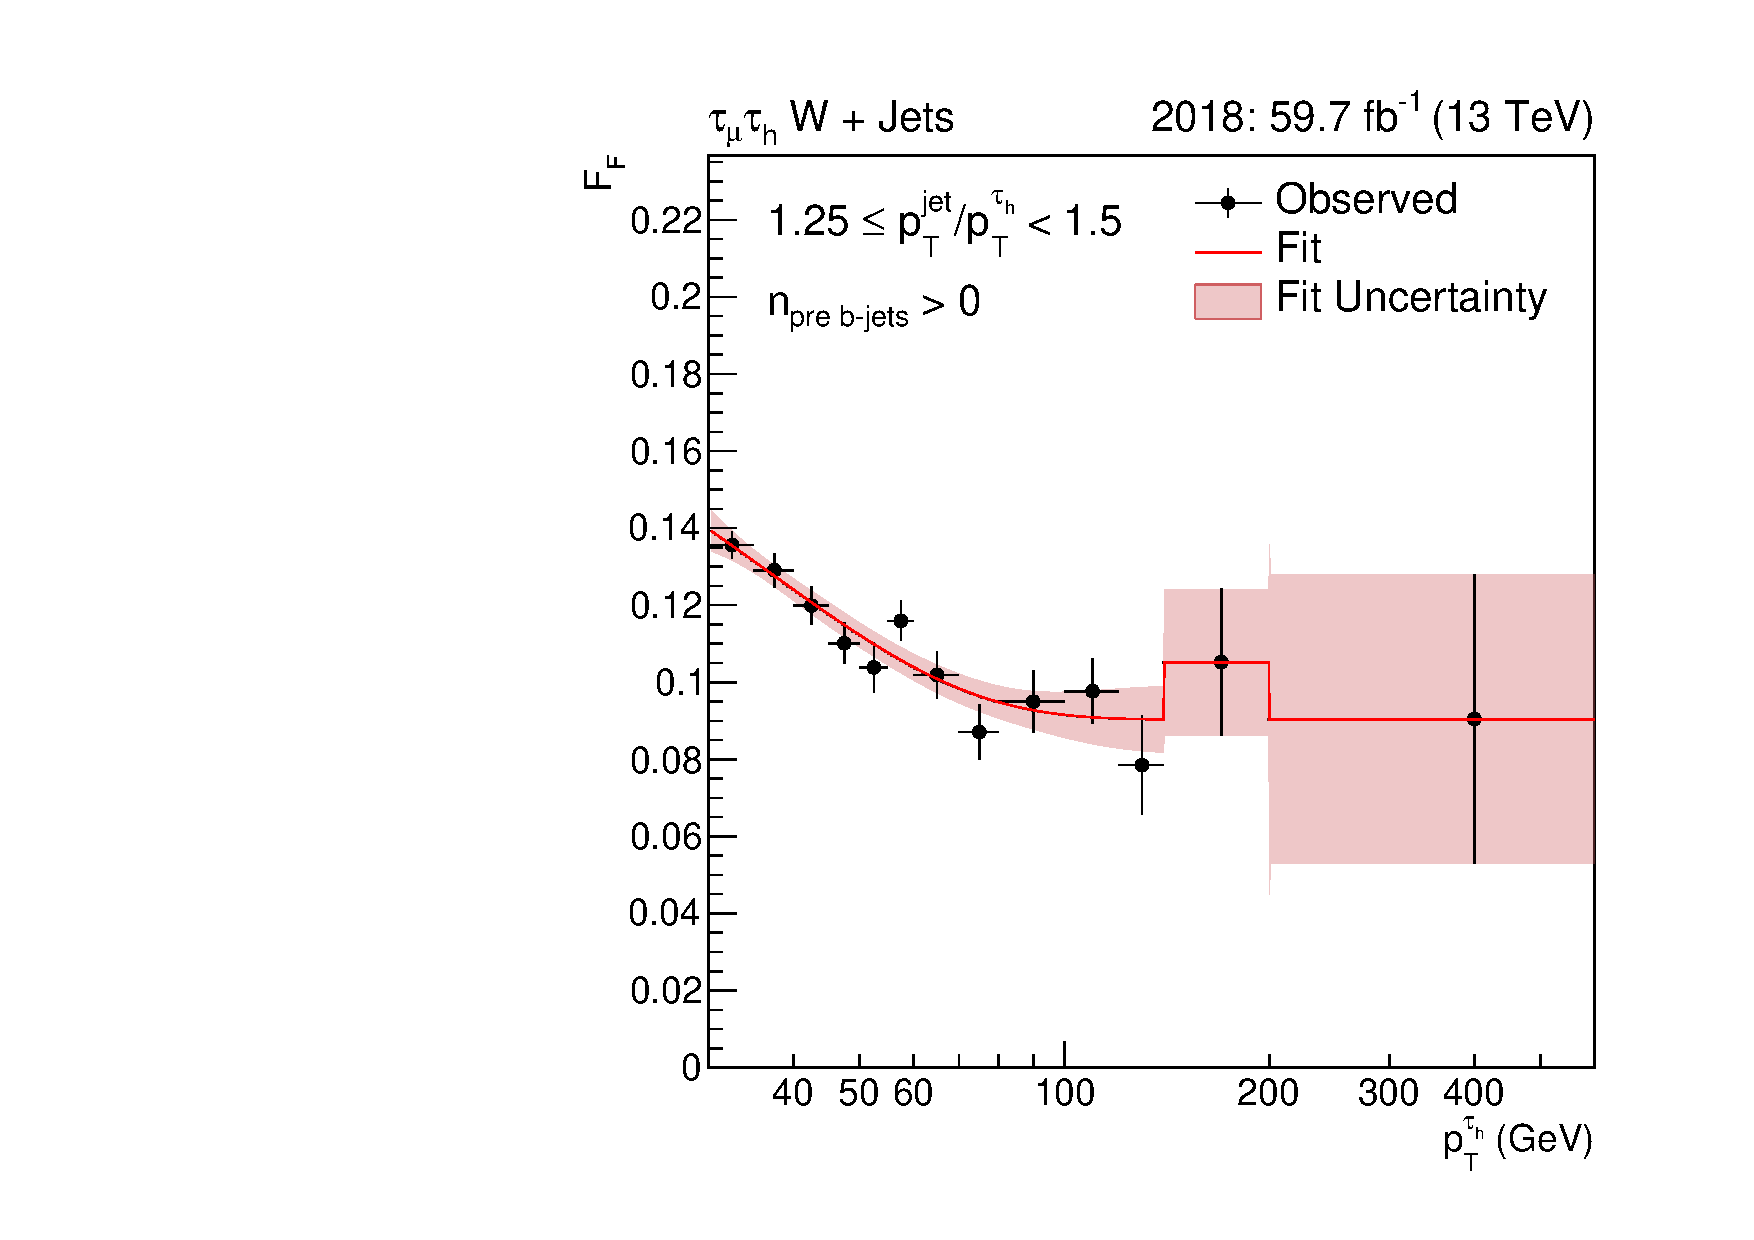
\includegraphics[width=.45\textwidth]{\PhDthesisdir/plots_and_images/from_CMS-NOTE-2020-218/ff_fit_jet_pt_med_1jet_pt_2_ff_wjets_mt_2018.tex}}
\hfill
\subcaptionbox{Ajustement de $\FF_t$.\label{subfig-chapter-HTT_analysis-section-bg_estimation-FF_method-ttbar}}[.45\textwidth]
{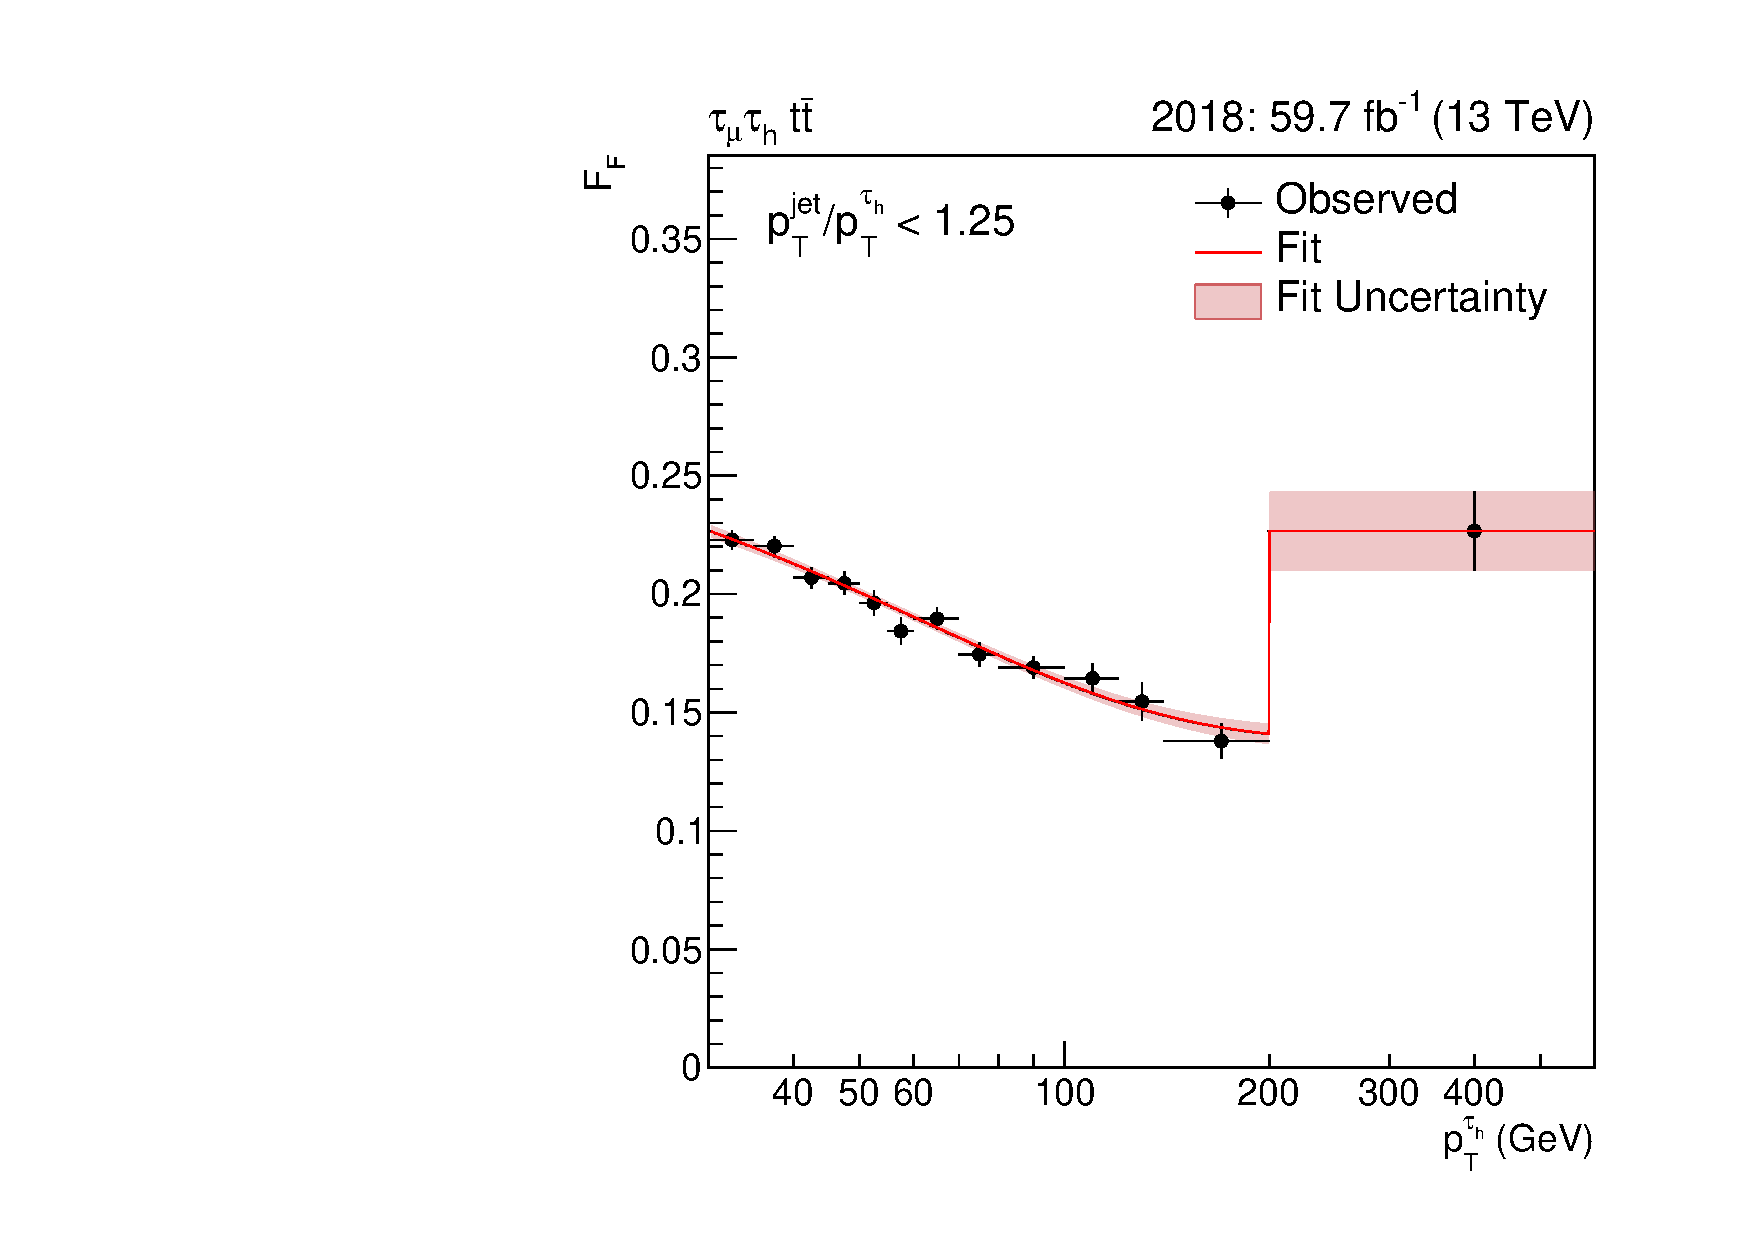
\includegraphics[width=.45\textwidth]{\PhDthesisdir/plots_and_images/from_CMS-NOTE-2020-218/ff_fit_jet_pt_low_inclusive_pt_2_ff_ttbar_mc_mt_2018.tex}}

\caption[Ajustements de $\FF_W$ et $\FF_t$ dans le canal \mu\tauh\ en 2018.]{Ajustements de $\FF_W$ et $\FF_t$ dans le canal \mu\tauh\ en 2018~\cite{CMS-NOTE-2020-218}.}
\label{fig-chapter-HTT_analysis-section-bg_estimation-FF_method-WJ-ttbar}
\end{figure}
\subsubsection{Corrections résiduelles}
Afin de valider les \fakefactors\ obtenus, ces derniers sont appliqués aux DRs pour les événements avec les mêmes points de fonctionnement de l'algorithme \DEEPTAU.
Les prédictions obtenues par les \fakefactors\ doivent alors correspondre aux observations brutes, \ie\ sans leur application.
Les écarts résiduels donnent la correction à appliquer, paramétrisée en fonction:
\begin{itemize}
\item du nombre de jets \Nprebjets\ identifiés comme issus de quarks~\quarkb, \Nbjets;
\item de l'impulsion transverse du lepton $\ell\in\set{\ele,\mu}$ pour les canaux semi-leptoniques, $\pT^{\ell}$;
\item de l'isolation du lepton $\ell\in\set{\ele,\mu}$ pour les canaux semi-leptoniques, $I^{\ell}$;
\item de la quantité d'énergie transverse manquante alignée avec le \tauh\ pour les événements QCD, $C_Q$,
\begin{equation}
C_Q = \frac{\MET}{\pT^{\tauh}} \cos(\Delta\phi(\vMET, \vpT^{\tauh}))
\mend[;]
\label{eq-FF_CQ_def}
\end{equation}
\item de la quantité d'énergie transverse manquante alignée avec le \tauh\ pour les événements \Wjets, $C_W$,
\begin{equation}
C_W = \frac{\norm{\vMET + \vpT^{\ell}}}{\pT^{\tauh}} \cos(\Delta\phi(\vMET + \vpT^{\ell}, \vpT^{\tauh}))
\mend[,]
\label{eq-FF_CW_def}
\end{equation}
dont la définition est semblable à celle de $C_Q$ mais où $\vMET$ est remplacé par $\vMET + \vpT^{\ell}$ afin de prendre en compte la contribution à \MET\ du neutrino issu de la désintégration du boson \Wboson.
Il est ici considéré comme dos-à-dos avec $\ell$, ce qui n'est strictement vrai que pour un \Wboson\ au repos.
\end{itemize}
%Les distributions de diverses variables, observées et prédites par les \fakefactors, doivent correspondre les unes aux autres.
%Les écarts résiduels entre observations et prédictions sont corrigées pour les variables qui n'ont pas encore été utilisées pour paramétriser les \fakefactors.
%\MET\ et $\pT^{\ell}$ observées et prédites par les \fakefactors\ doivent correspondre les unes aux autres.
%Les différences résiduelles sont alors corrigées.
%\par
%Les valeurs de \MET\ utilisées pour $\FF_Q$ sont corrigées en fonction de $C_Q$, définie équation~\eqref{eq-FF_CQ_def}.
%La correction est obtenue par un ajustement polynomial aux différences observées pour $\Nprebjets=0$ et $\Nprebjets\geq1$.
%Dans le cas de $\FF_W$ et $\FF_t$, les  valeurs de \MET\ utilisées sont corrigées en fonction de $C_W$, définie équation~\eqref{eq-FF_CW_def}.
%Un ajustement polynomial est réalisé dans les cas $\Nprebjets=0$ et $\Nprebjets\geq1$ pour $\FF_W$ et dans le cas général ($\Nprebjets\geq0$) pour $\FF_t$.
%\par
%Une fois les  valeurs de \MET\ corrigées, les distributions de $\pT^{\ell}$ le sont également pour $\FF_W$ et $\FF_t$.
Deux de ces corrections résiduelles obtenues sur le canal \mu\tauh\ en 2018 sont illustrées sur la figure~\ref{fig-chapter-HTT_analysis-section-bg_estimation-FF_method-closure}.
\begin{figure}[h]
\centering

\subcaptionbox{En fonction de $I_\mathrm{rel}^{(\mu)}$ pour $\FF_Q$.\label{subfig-chapter-HTT_analysis-section-bg_estimation-FF_method-closure-Q}}[.45\textwidth]
{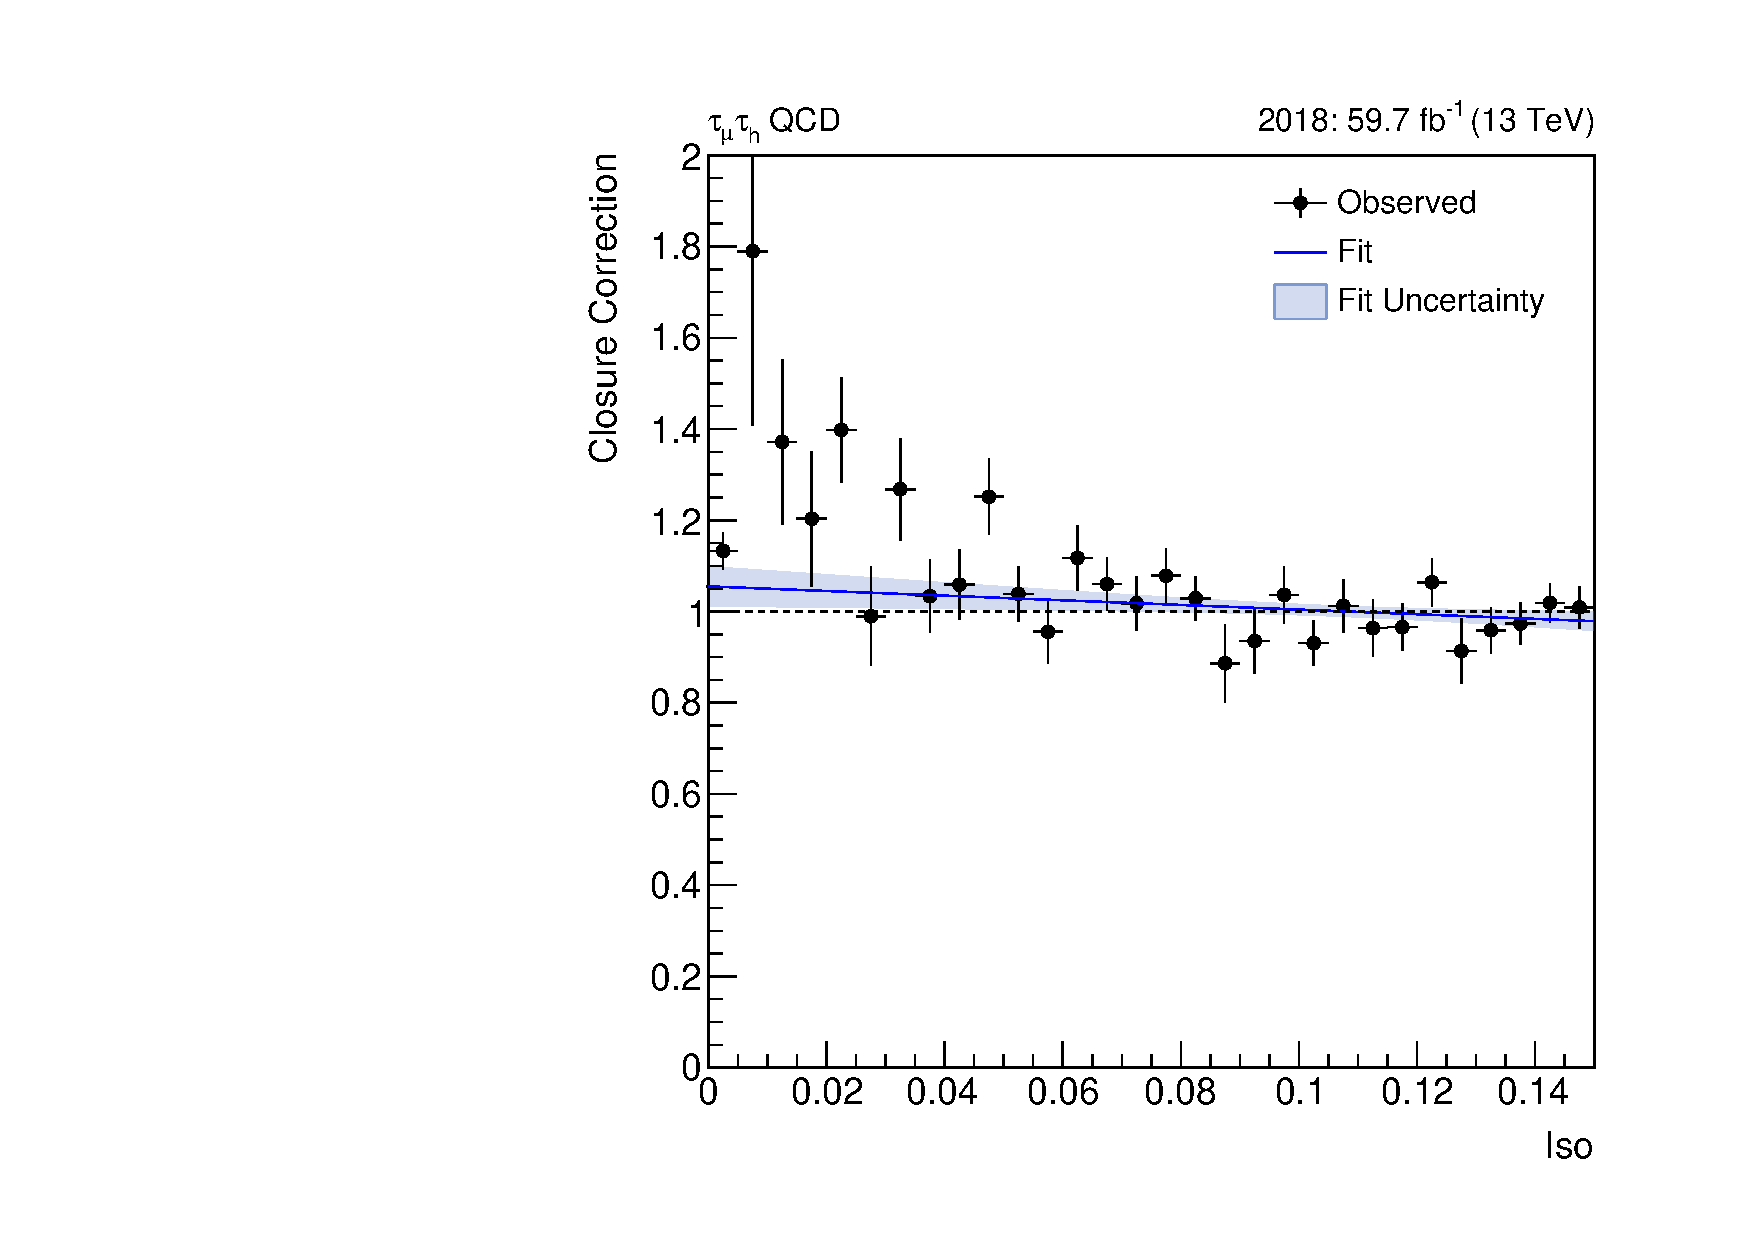
\includegraphics[width=.45\textwidth]{\PhDthesisdir/plots_and_images/from_CMS-NOTE-2020-218/ff_closure_iso_inclusive_closure_qcd_alt_mt_2018.tex}}
\hfill
\subcaptionbox{En fonction de $C_W$ pour $\FF_W$\label{subfig-chapter-HTT_analysis-section-bg_estimation-FF_method-closure-W}}[.45\textwidth]
{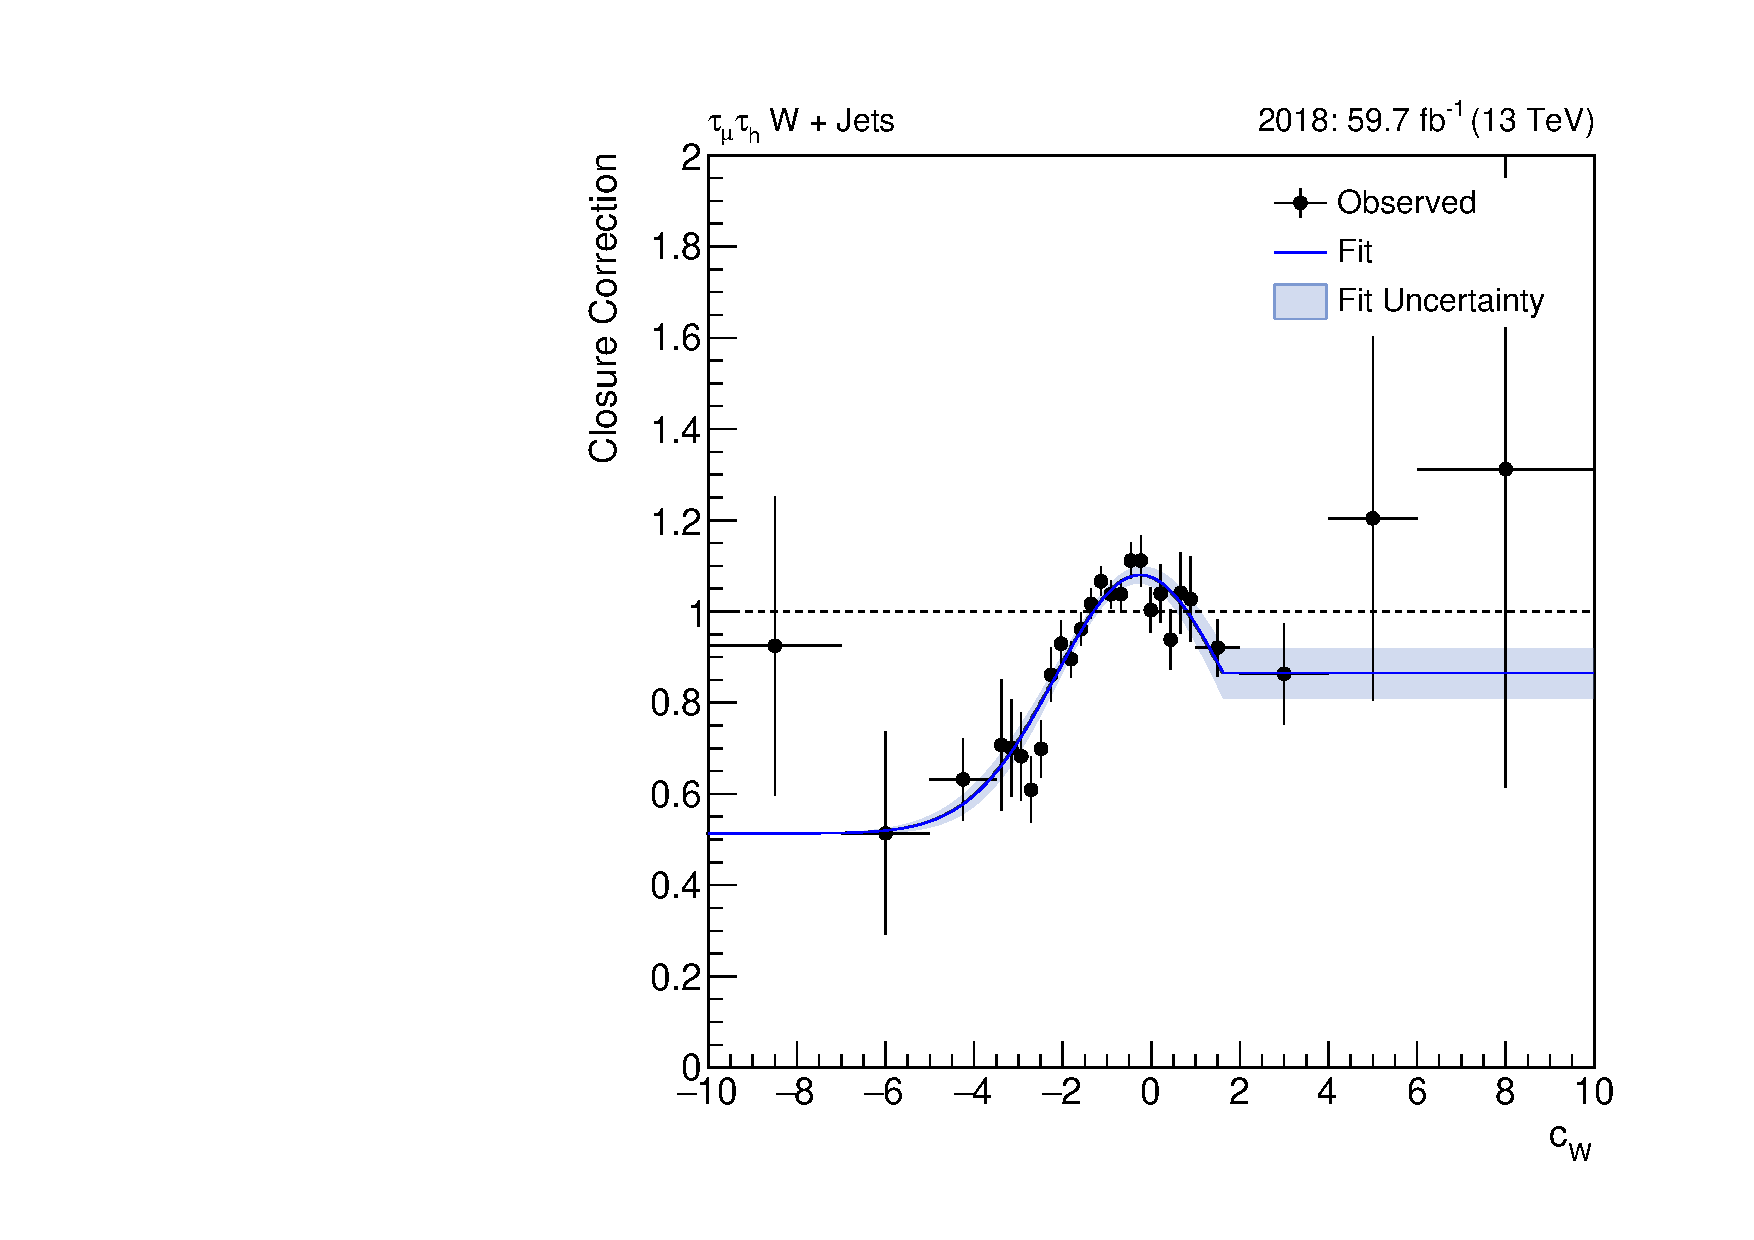
\includegraphics[width=.45\textwidth]{\PhDthesisdir/plots_and_images/from_CMS-NOTE-2020-218/ff_closure_met_1jet_closure_wjets_mt_2018.tex}}

\caption[Corrections résiduelles des \fakefactors\ dans le canal \mu\tauh\ en 2018.]{Corrections résiduelles des \fakefactors\ dans le canal \mu\tauh\ en 2018~\cite{CMS-NOTE-2020-218}.}
\label{fig-chapter-HTT_analysis-section-bg_estimation-FF_method-closure}
\end{figure}
\par
L'amélioration de la description des données ainsi obtenue grâce aux \fakefactors\ est visible sur la figure~\ref{fig-chapter-HTT_analysis-section-bg_estimation-FF_method-2018et_mT1_illustration}, où les distributions de la masse transverse de l'électron dans le canal \ele\tauh\ dans les données et dans l'estimation du bruit de fond sans et avec cette méthode sont tracées à titre d'illustration.
Outre un meilleur accord entre observations et estimation du bruit de fond, l'incertitude statistique est également réduite.
\begin{figure}[h]
\centering

\subcaptionbox{Sans \fakefactors.}[.475\textwidth]
{\plotHTTcontrol{2018}{emb_classic}{et}{mt_1_puppi}}
\hfill
\subcaptionbox{Avec \fakefactors.}[.475\textwidth]
{\plotHTTcontrol{2018}{emb_ff}{et}{mt_1_puppi}}

\caption{Distributions de la masse transverse de l'électron pour le canal \ele\tauh\ en 2018.}
\label{fig-chapter-HTT_analysis-section-bg_estimation-FF_method-2018et_mT1_illustration}
\end{figure}